\section{Motivation}

Let us first motivate the model presented herein. Suppose we are interested in drawing inferences from a system which is not directly observable. 

In particular, let us assume that the system comprises $m \in \nn$ states between which it switches. The state the system is in at time $t \in \nn$ is given by the value (in $\left(1, \dots, m\right)$) the random variable $C_t$ assumes. Hence, the behaviour of the system through time can be described as a \textit{process} $\left(C_1, C_2, \dots \right)$. As those states cannot be observed, they are also referred to as \textit{hidden states}. 

At each point of time, the system emits an \textit{observation}, which can be observed. The state the system is it at any given time governs which value is emitted at that time. Hence, each state has an associated distribution, according to which the observations are distributed. Let us denote the observation at time $t \in \nn$ by $X_t$. Then, analogously to the sequence of states, we have a sequence of observations $\left(X_1, X_2, \dots \right)$ where $X_t$ is distributed according to the distribution indicated by $C_t$. 

The aim of the algorithms developed throughout this dissertation is to draw inferences on the transitions between states, the sequence of the hidden states themselves  and the parameters describing their respective distributions. 






\section{Definition}


A \textit{Hidden Markov Model} (abbrev.: HMM) - for the purposes of this dissertation - comprises the following: 
\begin{itemize}
\item an unobservable, discrete-time, discrete-space time-homogeneous \textit{Markov Process} 
$\left(C_1, C_2, \dots \right)$ with $m \in \nn$ distinct hidden states.\\
The states' realisations determine the observations' distributions. 

\item a transition probability matrix (abbrev.: tpm) $\tpm \in \R_+^{m \times m}$ governing the state transitions of the Markov Chain. The tpm exhaustively describes $\prob{C_{t+1}}{C_t}$\footnote{The tpm is independent of $t$, hence \textit{time-homogeneous}. $C_t$ depends only on one previous time-step, which is why this process is named \textit{Markov Process}}.  

\item observable random variables $X_1, X_2, \dots$. The random variable $X_t$ is distributed as the distribution indicated by $C_t$. In particular, their distribution depends \textit{only} on an unobservable state. 
\end{itemize}
Without loss of generality we shall assume that $(C_t)$ is indexed by $\nn$. 


Note that while $\tpm$ describes the probability $\prob{C_{t+1}}{C_t}$, it does not give us any information on the \textit{initial distribution} of the chain, i.e. on $C_1$. Let us denote this initial distribution by  $\delta \in [0,1]^m$ with $\sum \delta_i = 1$. A common choice is the so-called \textit{stationary distribution}, which we shall explain later on. 

We shall use $\lambda$ to parameterise the states' distributions and use $\Theta := \left(\delta, \lambda, \Gamma \right)$ to describe all parameters of the model.

Furthermore, denote $\left(C_1, C_2, \dots, C_T \right)$ as $C^{(T)}$, $\left(C_1, C_2, \dots \right)$ as $\allC$, $\left(X_1, X_2, \dots, X_T \right)$ as $X^{(T)}$ and $\left(X_1, X_2, \dots \right)$ as $\allX$. 

The intuitive definitions above can be described mathematically as follows:
\begin{itemize}	
	\item $\prob{C_{t+1}}{\Theta, \allX, \allC} = \prob{C_{t+1}}{C_t}$
	
	\item $\prob{C_{t+1} = i}{C_t = j} = \tpm_{i, j} $ 
	
	\item $\prob{X_t}{ \Theta, \allX, \allC} = \prob{X_t}{C_t}$
\end{itemize}


The dependencies can easily be visualised in the following way:
\begin{figure}[H]
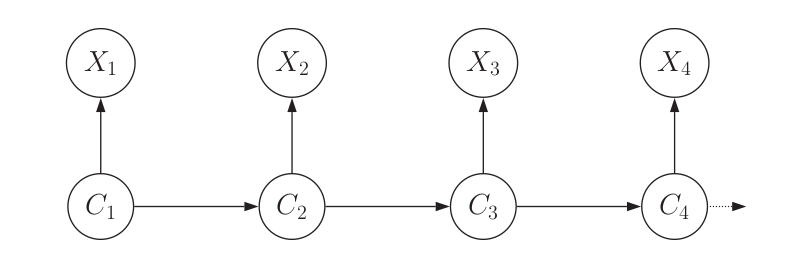
\includegraphics[width=0.8\linewidth]{img/hmm_dependencies.png}
\caption{Graph of dependencies within an HMM; figure as featured in Zucchini \cite{zucchini}}
\end{figure}
Here, each circle represents a random variable and each arrow a conditional dependency. In particular, each variable is conditionally independent of all other variables, if it is conditioned on the variable it is connected to in this graph. 


\section{Aim}
The aim of this dissertation is to compare two MCMC algorithms used to estimate the parameters of an HMM; namely Metropolis Hastings and Gibb's Sampler. We seek to practically compare both algorithms rather than employ theory to argue about their respective advantages. In particular, we are interested in the dependency of the requried number of iterations and running time on the complexity of the model as well as the sample size. 

Although there is an abundance of research on both Metropolis Hastings and Gibb's sampler, there is a lack of direct comparisons of both methods. However, related comparisons have been drawn; for instance Ryden\cite{ryden} compared the EM algorithm with MCMC methods. 

For instance, we would like to empirically answer the following questions:
\begin{itemize}
	\item How many samples does one need to reliably estimate a model of a given complexity?
	\item Which algorithm converges faster towards the true model?
	\item How does runtime depend on the model complexity?
	\item Do both algorithms produce chains of comparable quality?
\end{itemize}

Note that due to time constraints it is beyond the scope of this thesis to compare the state-of-the-art for both algorithms - implementing the state-of-the-art itself would be an undertaking worth of a dissertation. Rather, this dissertation compares both algorithms on a more foundational basis, which is unlikely to fundamentally change when algorithms are tweaked to achieve state-of-the-art performance. 



\section{Stationarity}
This section explains an effect of Markov Chains known as \textit{stationarity}. In particular, under a set of rather weak constraints\cite{mcnotes}, there exists a unique, discrete probability distribution $\pi \in \R_+^m$ named the \textit{stationary distribution}, with the following properties:
\begin{align*}
	\pi \Gamma &= \pi \\
	P(C_t = i) &\overset{t \rightarrow \infty}{\longrightarrow} \pi_i \quad \forall 1 \leq i \leq m \\
\end{align*}

The former condition states that when $P(C_t) \sim \pi \implies P(C_{t+1}) \sim \pi$ with $\prob{C_{t+1 = j}}{C_t = i} = \Gamma_{i, j}$ as usual. Hence, $\pi$ is \textit{invariant} under $\Gamma$ - when the chain is at a point where the states are assumed with a probability given by the stationary distribution, the states' probabilities do not change with a step in time. 

The latter property states that the chain converges towards its stationary distribution as $t \rightarrow \infty$. 

For details on the conditions and a proof, please refer to Breuer\cite{intro_processes}.
